% +--------------------------------------------------------------------+
% | Sample Chapter 2
% +--------------------------------------------------------------------+

\cleardoublepage

% +--------------------------------------------------------------------+
% | Replace "This is Chapter 2" below with the title of your chapter.
% | LaTeX will automatically number the chapters.                      
% +--------------------------------------------------------------------+

\chapter{Background}
\label{makereference2}

Two pieces of apparatus were used to conduct the experiments in this thesis. This chapter will detail the purpose, design and recreation of the equipment. Section ~\ref{makereference2.1} will cover the new Motorlab, including the hardware implementation, design of components, and basic functionality. Section ~\ref{makereference2.1} will also detail how a new type of position sensor works that is used for the position measurements of the Motorlab. Then, the older Motorlab will be discussed and compared to the new Motorlab in section ~\ref{makereference2.2}.

\section{New Motorlab}
\label{makereference2.1} 

The new Motorlab is experimental equipment that allows users to connect the theoretical ideas of control theory with those in practice. There are three main pieces of hardware that comprise the new Motorlab, namely the STM32 Nucleo, insert name here and insert name here. The STM32 Nucleo is an ARM based microcontroller that has pin headers for Arduino shields and other STM breakout boards. The Nucleo is the main development board of the new Motorlab


\subsection{Motorlab Parts}
\label{makereference2.1.1} 

\subsection{Position Sensor}
\label{makereference2.1.2} 

\begin{figure}[htb]%t=top, b=bottom, h=here

    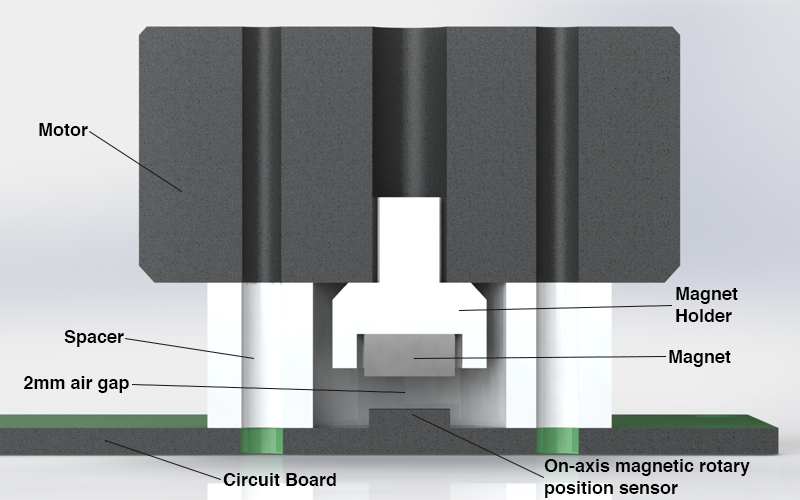
\includegraphics[height=4in]{figures/section_view_motorlab_assembly.png}

    \caption[Optional: Section View of Motorlab Assembly]{Section View of Motorlab Assembly}

    \label{figure1}
\end{figure}


\section{Old Motorlab}
\label{makereference2.2} 

Need information here